%File: anonymous-submission-latex-2024.tex
\documentclass[letterpaper]{article} % DO NOT CHANGE THIS

% AAAI packages
\usepackage{aaai24}  % DO NOT CHANGE THIS
\usepackage{times}  % DO NOT CHANGE THIS
\usepackage{helvet}  % DO NOT CHANGE THIS
\usepackage{courier}  % DO NOT CHANGE THIS
\usepackage[hyphens]{url}  % DO NOT CHANGE THIS
\usepackage{graphicx} % DO NOT CHANGE THIS
\urlstyle{rm} % DO NOT CHANGE THIS
\def\UrlFont{\rm}  % DO NOT CHANGE THIS
\usepackage{natbib}  % DO NOT CHANGE THIS AND DO NOT ADD ANY OPTIONS TO IT
\usepackage{caption} % DO NOT CHANGE THIS AND DO NOT ADD ANY OPTIONS TO IT
\frenchspacing  % DO NOT CHANGE THIS
\setlength{\pdfpagewidth}{8.5in} % DO NOT CHANGE THIS
\setlength{\pdfpageheight}{11in} % DO NOT CHANGE THIS
%
% These are recommended to typeset algorithms but not required. See the subsubsection on algorithms. Remove them if you don't have algorithms in your paper.
\usepackage{algorithm}
\usepackage{algorithmic}
% \usepackage{subcaption}
\usepackage{graphicx,subcaption}
\usepackage{adjustbox}
%
% These are are recommended to typeset listings but not required. See the subsubsection on listing. Remove this block if you don't have listings in your paper.
\usepackage{newfloat}
\usepackage{listings}


\DeclareCaptionStyle{ruled}{labelfont=normalfont,labelsep=colon,strut=off} % DO NOT CHANGE THIS
\lstset{%
	basicstyle={\footnotesize\ttfamily},% footnotesize acceptable for monospace
	numbers=left,numberstyle=\footnotesize,xleftmargin=2em,% show line numbers, remove this entire line if you don't want the numbers.
	aboveskip=0pt,belowskip=0pt,%
	showstringspaces=false,tabsize=2,breaklines=true}
\floatstyle{ruled}
\newfloat{listing}{tb}{lst}{}
\floatname{listing}{Listing}
%
% Keep the \pdfinfo as shown here. There's no need
% for you to add the /Title and /Author tags.
\pdfinfo{
/TemplateVersion (2024.1)
}

% DISALLOWED PACKAGES
% \usepackage{authblk} -- This package is specifically forbidden
% \usepackage{balance} -- This package is specifically forbidden
% \usepackage{color (if used in text)
% \usepackage{CJK} -- This package is specifically forbidden
% \usepackage{float} -- This package is specifically forbidden
% \usepackage{flushend} -- This package is specifically forbidden
% \usepackage{fontenc} -- This package is specifically forbidden
% \usepackage{fullpage} -- This package is specifically forbidden
% \usepackage{geometry} -- This package is specifically forbidden
% \usepackage{grffile} -- This package is specifically forbidden
% \usepackage{hyperref} -- This package is specifically forbidden
% \usepackage{navigator} -- This package is specifically forbidden
% (or any other package that embeds links such as navigator or hyperref)
% \indentfirst} -- This package is specifically forbidden
% \layout} -- This package is specifically forbidden
% \multicol} -- This package is specifically forbidden
% \nameref} -- This package is specifically forbidden
% \usepackage{savetrees} -- This package is specifically forbidden
% \usepackage{setspace} -- This package is specifically forbidden
% \usepackage{stfloats} -- This package is specifically forbidden
% \usepackage{tabu} -- This package is specifically forbidden
% \usepackage{titlesec} -- This package is specifically forbidden
% \usepackage{tocbibind} -- This package is specifically forbidden
% \usepackage{ulem} -- This package is specifically forbidden
% \usepackage{wrapfig} -- This package is specifically forbidden
% DISALLOWED COMMANDS
% \nocopyright -- Your paper will not be published if you use this command
% \addtolength -- This command may not be used
% \balance -- This command may not be used
% \baselinestretch -- Your paper will not be published if you use this command
% \clearpage -- No page breaks of any kind may be used for the final version of your paper
% \columnsep -- This command may not be used
% \newpage -- No page breaks of any kind may be used for the final version of your paper
% \pagebreak -- No page breaks of any kind may be used for the final version of your paperr
% \pagestyle -- This command may not be used
% \tiny -- This is not an acceptable font size.
% \vspace{- -- No negative value may be used in proximity of a caption, figure, table, section, subsection, subsubsection, or reference
% \vskip{- -- No negative value may be used to alter spacing above or below a caption, figure, table, section, subsection, subsubsection, or reference

\setcounter{secnumdepth}{0} %May be changed to 1 or 2 if section numbers are desired.

% The file aaai24.sty is the style file for AAAI Press
% proceedings, working notes, and technical reports.
%

% Title

% Your title must be in mixed case, not sentence case.
% That means all verbs (including short verbs like be, is, using,and go),
% nouns, adverbs, adjectives should be capitalized, including both words in hyphenated terms, while
% articles, conjunctions, and prepositions are lower case unless they
% directly follow a colon or long dash
\title{Interactive Visual Task Learning for Robots}
\author{
    % Authors
    Weiwei Gu,
    Anant Sah, 
    Nakul Gopalan
}
\affiliations{
    %Afiliations
    %\textsuperscript{\rm 1}Association for the Advancement of Artificial Intelligence\\
    % If you have multiple authors and multiple affiliations
    % use superscripts in text and roman font to identify them.
    % For example,

    % Sunil Issar\textsuperscript{\rm 2},
    % J. Scott Penberthy\textsuperscript{\rm 3},
    % George Ferguson\textsuperscript{\rm 4},
    % Hans Guesgen\textsuperscript{\rm 5}
    % Note that the comma should be placed after the superscript

    % Affiliations
    School of Computing and Augmented Intelligence, Arizona State University \\
    \{weiweigu, asah4, ng\}@asu.edu
%
% See more examples next
}

%Example, Single Author, ->> remove \iffalse,\fi and place them surrounding AAAI title to use it
\iffalse
\title{My Publication Title --- Single Author}
\author {
    Author Name
}
\affiliations{
    Affiliation\\
    Affiliation Line 2\\
    name@example.com
}
\fi

\iffalse
%Example, Multiple Authors, ->> remove \iffalse,\fi and place them surrounding AAAI title to use it
\title{My Publication Title --- Multiple Authors}
\author {
    % Authors
    First Author Name\textsuperscript{\rm 1},
    Second Author Name\textsuperscript{\rm 2},
    Third Author Name\textsuperscript{\rm 1}
}
\affiliations {
    % Affiliations
    \textsuperscript{\rm 1}Affiliation 1\\
    \textsuperscript{\rm 2}Affiliation 2\\
    firstAuthor@affiliation1.com, secondAuthor@affilation2.com, thirdAuthor@affiliation1.com
}
\fi




% These are our packages Nakul
\usepackage{booktabs}
\usepackage{xcolor}
\newcommand{\ngnote}[1]{\textcolor{blue}{\textbf{NG: #1}}}
\newcommand{\wgnote}[1]{\textcolor{red}{\textbf{WG: #1}}}
\newcommand{\asnote}[1]{\textcolor{orange}{\textbf{AS: #1}}}

\usepackage{enumitem}
% \usepackage{balance}




% REMOVE THIS: bibentry
% This is only needed to show inline citations in the guidelines document. You should not need it and can safely delete it.
\usepackage{bibentry}
% END REMOVE bibentry

\begin{document}

\maketitle


\begin{abstract}
We present a framework for robots to learn novel visual concepts and tasks via in-situ linguistic interactions with human users. Previous approaches have either used large pre-trained visual models to infer novel objects zero-shot, or added novel concepts along with their attributes and representations to a concept hierarchy. We extend the approaches that focus on learning visual concept hierarchies by enabling them to learn novel concepts and solve unseen robotics tasks with them.  To enable a visual concept learner to solve robotics tasks one-shot, we developed two distinct techniques. 
%\wgnote{This sentence seems awkward}
Firstly, we propose a novel approach, Hi-Viscont(HIerarchical VISual CONcept learner for Task), which augments information of a novel concept to its parent nodes within a concept hierarchy. 
% to a previously existing framework that represents concepts under a concept hierarchy.
%Firstly, our approach, Hi-Viscont(HIerarchical VISual CONcept learner for Task), represents  concepts under a concept hierarchy similar to previous approaches, with the additional ability to pass information to parent nodes. 
This information propagation allows all concepts in a hierarchy to update as novel concepts are taught in a continual learning setting. 
% namely Hi-Viscont(HIerarchical VISual CONcept learner for Task). 
% This ability is important in continual robotics settings allowing robots to categorize novel objects under known classes even with distinct visual features. 
Secondly, we represent a visual task as a scene graph with language annotations, allowing us to create novel permutations of a demonstrated task zero-shot in-situ. 
% The ability to represent tasks as a scene graph and the language annotations allows us . 
We present two sets of results. 
Firstly, we compare Hi-Viscont with the baseline model (FALCON~\cite{mei2022falcon}) on visual question answering(VQA) in three domains. 
%\wgnote{Fix the claim as follows}
While being comparable to the baseline model on leaf level concepts, Hi-Viscont achieves an improvement of over $9\%$ on non-leaf concepts on average.
%Hi-Viscont improves the f1 score from the baseline model by at least $1.7\%$ in each of the three domains on VQA with significance. 
Secondly, we conduct a human-subjects experiment where users teach our robot visual tasks in-situ. We compare our model’s performance against the baseline FALCON model. 
Our framework achieves $33\%$ improvements in success rate metric, and $19\%$ improvements in the object level accuracy compared to the baseline model.
With both of these results we demonstrate the ability of our model to learn tasks and concepts in a continual learning setting on the robot. 
\end{abstract}

\section{Introduction}
\section{Introduction}
Justice et al. \cite{justiceguide} state in their book that ``Children develop their knowledge of the world around them as they interact with their environment directly and indirectly. The direct experiences children have in their homes, schools and communities certainly provide the greatest amount of input to the world knowledge base.''. This knowledge arises from both physical and conversational interactions. In this paper, we test the hypothesis that just like a human child, machines need interaction to acquire world knowledge and develop commonsense reasoning abilities, and we study the effect of conversational interactions on this knowledge acquisition. Most of the literature on commonsense reasoning 
relies %rely [kmm- most-> relies]
on extracting the largest possible snapshot of 
%the [kmm- removed]
world knowledge and either 
query %query [kmm- on-> extracting and querying]
it or 
propose %propose [kmm- most-> proposes][could also parse as 'relies on-> proposing' or 'querying or proposing', may be better to restructure the sentence][fa- it was the later, so i restructured]
automated knowledge base completion methods for it. We argue that it is necessary to equip reasoning engines with an interaction strategy facilitating the extraction of just-in-time information needed for reasoning. 
%, through conversation with a human user [kmm- removed; conversation is covered by 'interaction' earlier in the sentence]
In this paper, we 
take up %take a few steps towards [kmm- rephrase (take steps/take steps repetitive)]
this grand goal, %[kmm- comma added]
and although we do not solve the whole challenge, we take the first steps needed for addressing it. 
Specifically, here we propose a ``soft'' commonsense reasoning engine and solve targeted knowledge base completion problems based on the information provided by the user through a conversational interface.

% We state this as our overarching grand research goal and mention carefully that we are taking a few steps towards this grand goal. Although it does not solve all of it but it is a step towards achieving this goal. This is just a first step however its a part of a very well reasoned and ambitious project. Then we also carefully describe the limitations of the project
% In other words, our overarching goal is having a human construct a reasoning system that does not have commonsense and extract commonsense from the user through conversation.
% \amoscomment{I think that it might be better saying something like: this work takes the first step towards ... I think that the paper could also benefit from adding a few sentences at the beginning.} \facomment{Is this resolved now?}

We believe that this is the right time for this proposal specifically since conversational agents such as Siri, Google home, Alexa and Cortana among others are starting to enter our daily lives. Therefore, it is plausible to assume that 
such agents %we [kmm- rephrase]
have access to conversation with a human for extracting commonsense knowledge. In this paper, we work with the Learning by Instruction Agent (LIA) \citep{azaria2016instructable,labutov2018lia} and develop a commonsense reasoning system for her called CORGI (\textbf{CO}mmonsense \textbf{R}easonin\textbf{G} by \textbf{I}nstruction). In what follows, we present our definition of commonsense reasoning for LIA after briefly introducing her. % It is worth noting, however, that the proposed method is not limited to a specific conversational agent. 
% \kmcomment{Anthropomorphizing LIA (referring to the agent as 'her') is a somewhat political choice -- it's okay to make it, but make it consciously.}

LIA is an intelligent agent that operates on 
a user's smartphone. %the phone [kmm- rephrase (you do not call LIA; there are other agents where you call in so it's important to make the distinction)]
%and can be taught new commands through user instructions. [kmm- removed (covered in the very next sentence)]
End users add new functionalities to LIA through verbal instructions and teach her how to perform new tasks. For example, the user can tell LIA, ``whenever it snows at night, wake me up 30 minutes early''. If LIA does not understand how to perform this task, she will ask the user to instruct her by breaking the task down into a set of steps in a teaching session. In this case, the user can say, ``(first) open the weather app, (second) see if the night weather condition is snow, (third) if true then adjust my alarm to 30 minutes earlier''. After this teaching session, LIA can perform this task. 

One phenomenon we have noticed in collecting these types of ``Whenever $S$ occurs, then do $A$'' instructions is that people often {\em underspecify} the precondition $S$. For example, one instructor might want to wake up early when it snows because they are concerned about getting to work on time.  For this user, the implied precondition is not really ``whenever it snows,'' but instead ``whenever it snows enough to cause traffic slowdowns, and it's a workday.'' The point is %Amos: I think that "the point is" doesn't sound good. How about "Naturally,"?
that people often fail to specify  such detailed conditions, perhaps because they are used to speaking to other people who possess the common sense needed to infer the more specific intent of the speaker.

Our goal for LIA is to use background commonsense knowledge to reason about the user's more specific intent, and to discuss this with the user in order to create the correct preconditions for the recommended action.  Therefore, we assume LIA can obtain statements from the user that fit the logical template ``Whenever $S$ occurs, do $A$ because I want to achieve goal $G$.''\footnote{Note in LIA's conversational setting, if the user gives an instruction of the form ``Whenever $S$ occurs, do $A$.'' and omits the reason, then LIA can simply respond ``Why do you want to do that?'' in order to prompt for the missing reason $G$.}
%LIA then generalizes from this statement to other actions. For example, if the user says, ``if the weather is rainy tomorrow then set an alarm for 1 hour later'', LIA can perform this action without needing to be taught again. However, this generalization has some limitations which 
%stem %stems [kmm- limitations->stem]
%from the lack of reasoning capabilities in LIA. 
For example consider the following two statements: %, [kmm- colon replaces comma]
\begin{itemize}
\item Whenever it snows at night, wake me up 30 minutes early because I don't want to be late to work
\item Whenever it snows at night, wake me up 30 minutes early because I have never seen the snow before 
\end{itemize}
Note that in the first statement, the user will not want to wake up early on a weekend or a holiday (assuming that they do not work then) whereas in the second scenario, the user will want to wake up early regardless of the date in order to see snow for the first time -- but might not want to wake up early once she has seen snow for the first time.

In CORGI, the role of commonsense reasoning is to derive the intended condition to use in place of the stated $S$ given an ``If $S$ then do $A$ because $G$'' statement from the user. Its general approach is to derive an explanation of how action $A$, performed in state $S$ will achieve goal $G$, and then to derive the intended precondition $S$ by collecting the preconditions on $S$ that allow this explanation to hold.  CORGI has access to a limited amount of general background knowledge about the world, represented in a logic programming language. Reasoning reduces to using this background knowledge to perform multi-hop logical inference. If no reasoning path is found, CORGI initiates a conversation with the user to extract relevant background knowledge and adds it to its underlying understanding of the world.  This newly acquired background knowledge will be used in future user interactions with CORGI. In essence, we are performing knowledge base completion through conversation, on a need-driven basis. Note that in earlier work Hixon et al. \cite{hixon2015learning} perform relation extraction using human interaction for question answering. Although the general idea of using human interaction is similar to our proposal, the information extraction method and the problem studied in \cite{hixon2015learning} differs from our setting. To the best of our knowledge, CORGI is the first conversational assistant that targets completing reasoning paths.
% \amoscomment{'their' seems like a typo, not sure what you are saying} --> resolved
% Therefore, our reasoning system is a commonsense reasoning by instruction engine. 

% \amoscomment{I find it hard to understand when 'LIA' refers to the agent from previous work, and when it refers to new capabilities added by this work.} \facomment{is this resolved now, Amos?} %Yes, Thanks!

% In this paper we develop a reasoning system for LIA that is capable of commonsense reasoning in order to generalize correctly given if-then user commands through the because statement.

CORGI's main reasoning component is the multi-hop inference system. Since the knowledge is represented in a logic programming language, the underlying inference algorithm is backward chaining. However, backward chaining in its traditional form is not robust to variations in natural language. This is specifically of importance since CORGI allows open-domain dialog with the user
to reduce the startup cost of the user having to learn a %so that the user is not limited to a [kmm- is this rephrase correct?]
specific grammar or vocabulary. Therefore, there is no parsing algorithm to resolve these variations. For example, in 
%the [kmm- removed]
traditional backward chaining, the statements ``if the forecast is snow tonight'' and ``if the weather is snowy tonight'' are thought of as two different statements whereas we want them both to map to the same representation. In order to address this, we propose a ``soft backward chaining'' algorithm that learns continuous representations or embeddings of the logical statements in the background knowledge. This will allow CORGI to indicate the equivalence of semantically similar statements based on the distance of their learned representations in the vector space. This soft backward chaining allows us to bridge a gap between symbolic AI and neural approaches using the best of both worlds.

% CORGI's soft backward chaining algorithm is end-to-end differentiable and is trained by looking at the proof traces of similar 

% kmm: resolve AA's confusion here with "compatible with deep-learning techniques"

% . This multi-hop reasoning system is end-to-end differentiable and supports soft multi-hop reasoning to account for natural language variations. \amoscomment{I might be missing something, but what does it mean being end-to-end differentiable, are you referring to differentiable functions (those that have a derivative), is this required in order to train the system? Or do you mean that the system obtains knowledge piece by piece. I guess you mean the former, but I did struggle with this.}

% \tmcomment{There are two main themes: 1. claiming that the reasoning can help get the generalization right, 2. how to do the reasoning in a way that is correct}

% \tmcomment{why are we doing reasoning this way and how can we make sure we can do it successfully. we need to compare it with the approximate inference and probabilistic inference methods for performing reasoning}

% \tmcomment{Our contributions are two fold. one is that we are proposing a reasoning strategy through conversation and are proposing to extract the missing information just in time to perform the correct reasoning. No one has the capacity to store the world's largest kb and until now everyone has tries to maintain the largest knowledge bases that there are. However, we are proposing a new way of doing this and it is to extract the correct part of the missing knowledge from the user. This is our grand goal and we have performed a set of small steps towards it... [layout the steps]. Another contribution is the soft unification part. In order to make this work we need to combine symbolic AI with neural approaches to bridge the gap and use the best of both worlds.}

% \tmcomment{reviewer question: How do we know if our method scales? No one has a large enough knowledge base that contains all the information there is in the world. And currently everyone in the field is trying to do this. However, we are proposing a method for extracting the right information just in time needed to perform the reasoning}

% \tmcomment{We do not know the user will give us the right answer even if we ask the right question} \kmcomment{Focus less on ``right'' answer/question here; there are many-to-many possible question/answer pairs that will give a good result. Make a definition of what success means in this context.}

% \tmcomment{Our goal is to have a conversation with the user and the main goal is to have the user give us the missing part of the information and in a funny/not so funny way this is a feature of the system}

% \tmcomment{consider the problem of learning procedures including triggers by conversation. When humans give instructions they are imprecise. In this project we are interested in having the human construct a reasoning system that does not have the commonsense and we want to use conversation to extract the commonsense from the user. We state this as our overarching grand research goal and mention carefully that we are taking a few steps towards this grand goal. Although it does not solve all of it but it is a step towards achieving this goal. This is just a first step however its a part of a very well reasoned and ambitious project. Then we also carefully describe the limitations of the project.}

\section{Related Work}

\textbf{Language conditioned manipulation.} 
Significant work has been performed in  learning concepts and tasks for robots in interactive settings~\cite{gopalan2018sequence,gopalan2020simultaneously,tellex2020robots} even with the use of dialog~\cite{chai2018language,matuszek2012joint}.
Our work differs from previous works as it learns visual concepts for manipulation one-shot, and improves generalization by updating other known concepts.
Moreover, our approach can learn a concept hierarchy starting from zero known concepts, displaying the adaptability of our model under a continual learning setup.
%Our work differs from previous works as it is attempting to learn visual concepts for manipulation one-shot, while updating other known concepts to improve generalization.
%Moreover, our approach is completely differentiable and can start with zero known concepts, which is important for a continual learning setup. 
Previous work has focused on language conditioned manipulation~\citep{shridhar2021cliport, liu2021structformer, brohan2023rt1, brohan2023rt2}. \citealt{shridhar2021cliport} computes a pick and place location conditioned on linguistic and visual inputs. 
\citealt{liu2021structformer} focuses on semantic arrangement on unseen objects. 
Other works train on large scale linguistic and visual data and can perform real-life robotic task based on language instructions~\citep{ahn2022i, brohan2023rt1, brohan2023rt2}. Our work focuses on interactive teaching of tasks and concepts instead of focusing on the emergent behaviors from large models. 
% \citealt{ahn2022i} uses a pre-trained to propose plans to complete task and executes the feasible grounded plan. 
% None of these approaches discussed above focus on one shot teaching of concepts and task types to solve novel tasks in a zero-shot setting.
\citealt{daruna2019robocse} learns a representation of a knowledge graph by predicting directed relations between objects allowing a robot to predict object locations. 
To the best of the author's knowledge, our work  is the first that learns concepts and tasks one-shot to generalize to novel task scenarios on a robot, making our contributions significant compared to other related works.   


\noindent\textbf{Visual reasoning and visual concept learning.} Our work is related to visual concept learning \citep{mei2022falcon, mao2018the, yi2019neuralsymbolic, han2020visual, li2020competenceaware} and visual reasoning \citep{Mascharka_2018, DBLP:journals/corr/abs-1807-08556, DBLP:journals/corr/JohnsonHMHLZG17, DBLP:journals/corr/abs-1803-03067}. To perform the visual reasoning task, traditional methods \citep{Mascharka_2018, DBLP:journals/corr/abs-1807-08556, DBLP:journals/corr/JohnsonHMHLZG17, DBLP:journals/corr/abs-1803-03067} decompose the visual reasoning task into visual feature extraction and reasoning by parsing the queries into executable neuro-symbolic programs.  On top of that, many concept learning frameworks \citep{mei2022falcon, mao2018the, yi2019neuralsymbolic, han2020visual, li2020competenceaware} learn the representation of concepts by aligning concepts onto objects in the visual scene. 
% \ngnote{\citealt{yi2019neuralsymbolic} parses the visual scene into a structural scene representation, which makes the results of the neural network more interpretable.  \citealt{mao2018the} presents a concept learner that jointly learns a visual feature extractor, visual concept representation, and semantic parsing. \citealt{han2020visual} shows that introducing the relationships between concepts and higher-level concepts is helpful in learning the concept’s representation. \citealt{mei2022falcon} even shows that it is possible to train a module that learns a new concept with a very limited number of examples and its conceptual relationship to known concepts.} 
As far as we know, \citealt{mei2022falcon}'s FALCON is the most similar work to our work in this line of research. However, when introducing a new concept, our work continually updates the representation of all related concepts, whereas \citealt{mei2022falcon} does not, which makes it ill-suited for continual learning settings. Our work is also related to the area of few-shot learning~\citep{snell2017prototypical, tian2020rethinking, vinyals2017matching}, which learns to recognize new objects or classes from only a few examples but does not represent a concept hierarchy which is useful in robotics settings.



% \textbf{Few-shot learning.} Our work is also related to the area of few-shot learning, which learns to recognize new objects or classes from only a few examples. \citealt{vinyals2017matching} and \citealt{snell2017prototypical} use the visual features of a small number of annotated images as representation for the new class. 
% While the existing frameworks use Euclidean distance or cosine similarity to compute similarity between classes, \citealt{sung2018learning} trains a learnable module to predict the similarity between examples. Provided the relationship between the new class and known class, \citealt{wang2018zeroshot} and Kampffmeyer et al. \cite{kampffmeyer2019rethinking} learn the representation of a new class with no visual example. \citealt{tian2020rethinking} trains a transferable embedding model that can generalize to new classes. 

% \textbf{Continual learning and knowledge graphs.} Another area of work related to ours is continual learning and knowledge graphs. \citealt{daruna2019robocse} learn a representation of a knowledge graph by predicting whether a directed edge between two vertices is within the graph or not. On top of the existing framework, \citealt{daruna2021continual} shows that it is possible to continually update the knowledge graph whenever a new edge or a new vertex appears while avoiding catastrophic forgetting. 

\noindent\textbf{Scene graph.} Scene graphs are  structural representations of all objects and their relationships within an image. The scene graph representation~\cite{Chang_2023} of images is widely used in the visual domains for various tasks, such as image retrieval\cite{DBLP:journals/corr/JohnsonHMHLZG17}, image generation\citep{johnson2018image}, and question answering\citep{teney2017graphstructured}.
This form of representation has also been used in the robotics domains 
% combines geometric scene graph and symbolic scene graph as a representation of the scene 
for long-horizon manipulation~\citep{zhu2021hierarchical}.


\section{Methods}
\section{Methods}

\subsection{Problem Formulation}
In crop yield prediction, we denote each county's climatic features by $\mathbf{x}_{c,t}$ and ground-truth crop yield (for a particular crop) by $y_{c,t}\in \mathbb{R}$, where $c$, $t$ represent county and year respectively. Each $\mathbf{x}_{c,t}$ contains four types of features (detailed descriptions of these features can be found in the Experiments section): weather features $\mathbf{x}_{c,t}^w\in \mathbb{R}^{n_w\times 52}$, land surface features $\mathbf{x}_{c,t}^l\in \mathbb{R}^{n_l\times 52}$, soil quality features $\mathbf{x}_{c}^s\in \mathbb{R}^{n_s\times 6}$, and some extra features (e.g. crop production index) $\mathbf{x}_{c}^e\in \mathbb{R}^{n_e}$. Namely, $\mathbf{x}_{c,t}=(\mathbf{x}_{c,t}^w, \mathbf{x}_{c,t}^l, \mathbf{x}_{c}^s, \mathbf{x}_{c}^e)$. We denote the number of weather, land surface, soil quality, and extra variables as  $n_w, n_l, n_s, n_e$ respectively. Among these features, $\mathbf{x}_{c,t}^w, \mathbf{x}_{c,t}^l$ change both spatially and temporally, while $\mathbf{x}_{c}^s, \mathbf{x}_{c}^e$ are county-specific and remain stable over time. The goal is to predict $y_{c,t}$ given $\mathbf{x}_{c,t}$. Recent work \cite{khaki2020cnn} also showed features from past years can help with the prediction, so we reformulate our task as predicting $y_{c,t}$ with $\{\mathbf{x}_{c,t},\mathbf{x}_{c,t-1},...,\mathbf{x}_{c,t-\Delta t}\}$. $\Delta t$ is the length of year dependency. If $\Delta t=0$, the model will not consider features from prior years. 

\subsection{Per-Year Embedding Extraction}
Regardless of whether the models use historical features or not, the first step is always to extract an embedding for each year from $\mathbf{x}_{c,t}$. Then a prediction can be made based on the embedding from the current year or the embeddings from the last few years.

The four types of features $\mathbf{x}_{c,t}^w, \mathbf{x}_{c,t}^l, \mathbf{x}_{c}^s, \mathbf{x}_{c}^e$ have different structures. Using a uniform neural network to extract the embedding may not effectively exploit the structure in the raw data. For example, weekly features $\mathbf{x}_{c,t}^w, \mathbf{x}_{c,t}^l$ naturally incorporate a temporal order, but county-specific soil features $\mathbf{x}_{c}^s$ do not change temporally and are measured at different depths underground. Therefore, we use separate neural networks to process the differently structured-parts from $\mathbf{x}_{c,t}$:
\begin{equation}
\label{eq:cnn}
\begin{aligned}
&\mathbf{h}_{c,t}^{wl}=f_{wl}(\mathbf{x}_{c,t}^w, \mathbf{x}_{c,t}^l) \\
&\mathbf{h}_{c}^s=f_s(\mathbf{x}_{c}^s) \\
&\mathbf{h}_{c,t}=(\mathbf{h}_{c,t}^{wl}, \mathbf{h}_c^s, \mathbf{x}_{c}^e)
\end{aligned}
\end{equation}
$f_{wl}(\cdot)$ handles the features that vary over time. Since land surface features like soil moisture from $\mathbf{x}_{c,t}^l$ are weekly data closely related to weather, we concatenate $\mathbf{x}_{c,t}^l$ and $\mathbf{x}_{c,t}^w$ before further passing to $f_{wl}$. Given the temporal order, an RNN or a CNN can be used for $f_{wl}$ to facilitate information aggregation along the time axis. On the other hand, $f_s(\cdot)$ aggregates information along soil depths. We use CNN as the architecture for $f_s$. $\mathbf{x}_{c}^e$ only contains six scalar values, so we directly pass it to the output embedding. The final embedding $\mathbf{h}_{c,t}$ is the concatenation of $\mathbf{h}_{c,t}^{wl}, \mathbf{h}_c^s, \mathbf{x}_{c}^e$.


\begin{figure*}[t]
\centering
\begin{minipage}[c]{7cm}
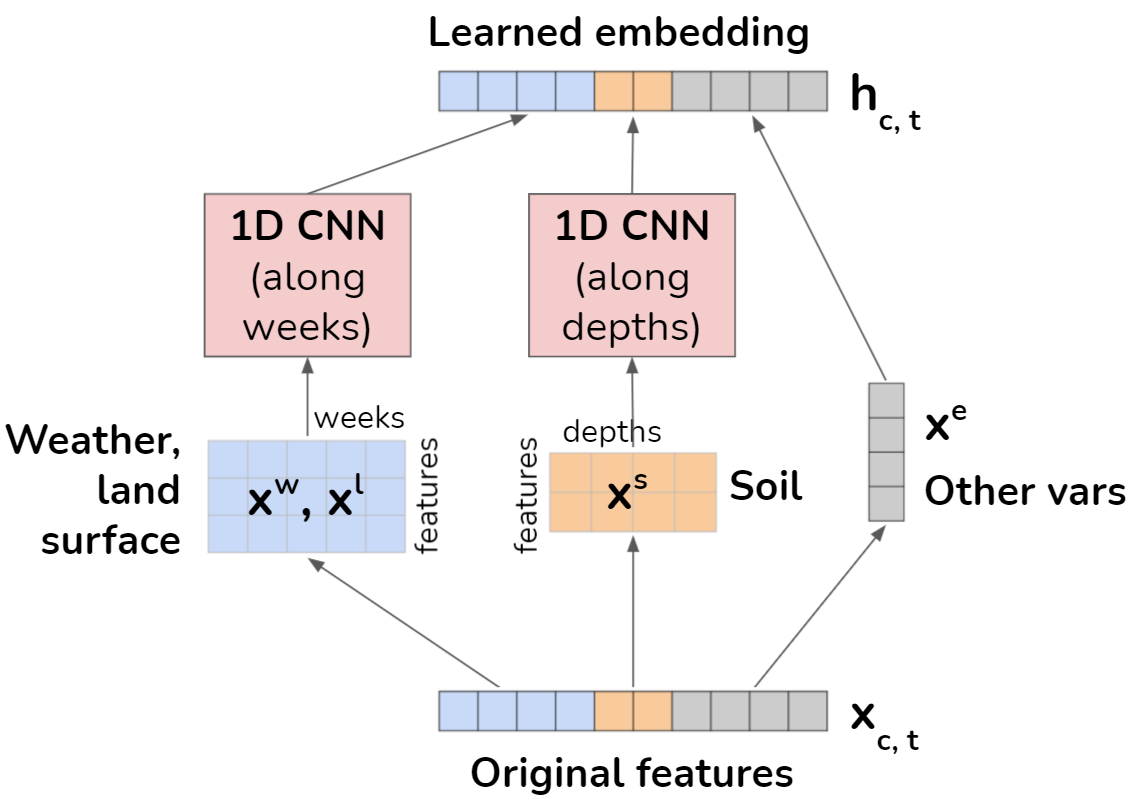
\includegraphics[width=6.9cm]{figs/cnn.png}
\label{fig:cnn}
\end{minipage}
\begin{minipage}[c]{10cm}
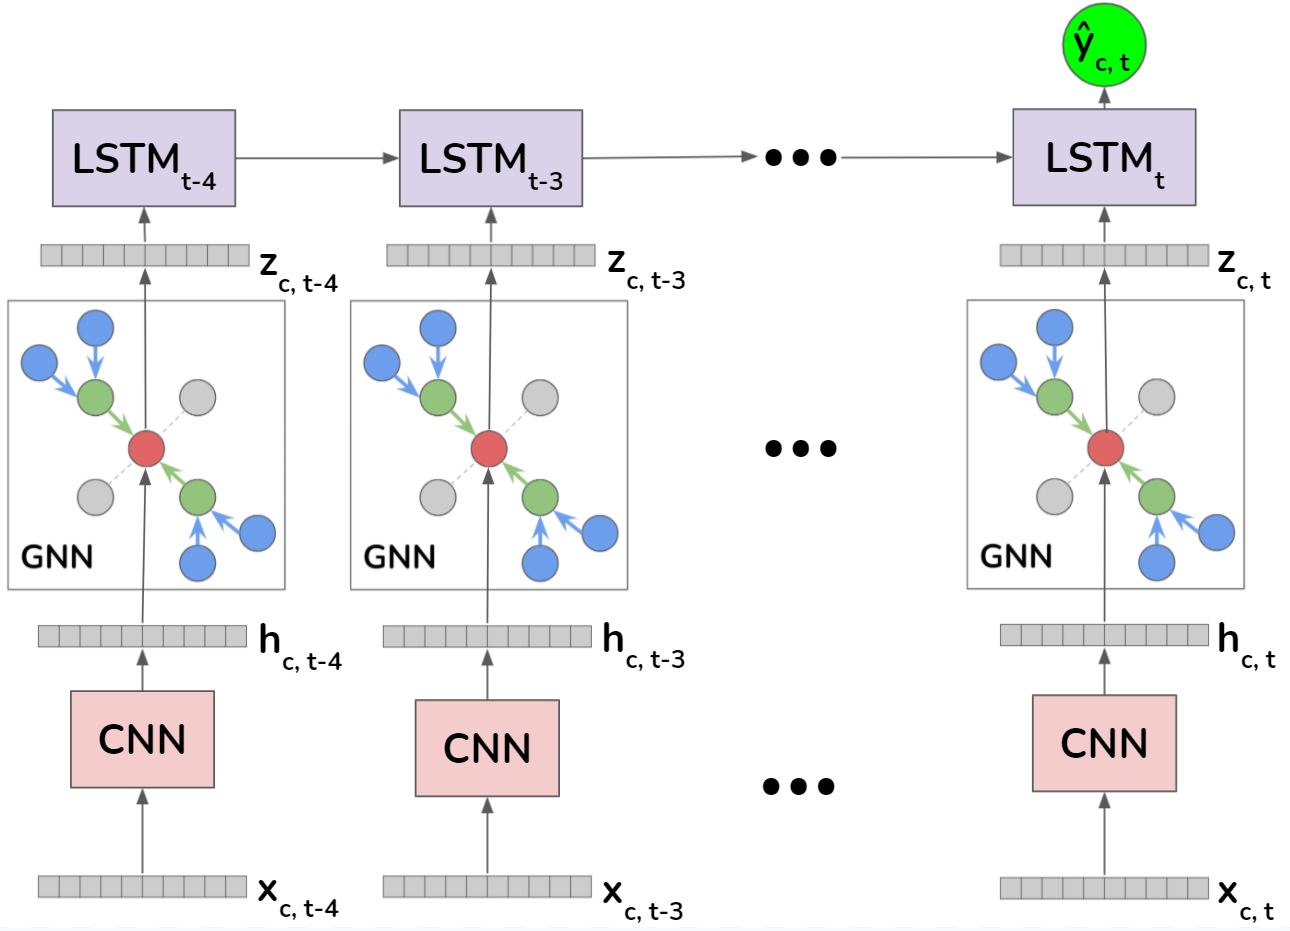
\includegraphics[width=9.9cm]{figs/gnn-rnn.png}
\label{fig:gnn-rnn}
\end{minipage}
\caption{\textbf{Left}: The CNN model used for per-year embedding extraction. \textbf{Right}: Our overall GNN-RNN framework. For each county $c$ and year $t'$, the CNN extracts an embedding $\mathbf{h}_{c, t'}$. Then we apply a GNN to refine each year's embedding by aggregating information from neighboring counties, producing a new embedding $\mathbf{z}_{c, t'}$. Finally, an LSTM processes the embeddings from each year and outputs the yield prediction $\widehat{y}_{c, t}$.}
\end{figure*}


\subsection{Temporal Dependency}
Though new crops are planted every year and yields primarily depend on climatic factors within one year, it has been observed that the trend and variations captured by recent history can be very informative for prediction \cite{khaki2020cnn}. For example, crop yields have tended to increase over the past few decades due to improvements in technology and genetics \cite{ortiz2018another}. While data on the underlying technological improvement is unavailable \cite{khaki2020cnn}, we can observe recent trends in crop yield. Our per-year embedding extraction makes it easy to incorporate  historical knowledge. All we need is an RNN that reads the per-year embeddings from the current year and several prior years. The output from the last time step would be our prediction for the crop yield of the current year: 
\begin{equation}
\label{eq:rnn}
\begin{aligned}
\widehat{y}_{c,t}=r(\mathbf{h}_{c,t-\Delta t}, ..., \mathbf{h}_{c,t-1}, \mathbf{h}_{c,t})
\end{aligned}
\end{equation}
where $r(\cdot)$ is an RNN, and $\mathbf{h}_{c,t'}$ is the embedding from year $t'$ for county $c$. The model described so far follows the CNN-RNN framework, which has previously been shown to outperform single-year NN models \cite{khaki2020cnn}.


\subsection{Incorporating Geographical Knowledge}
Eq.~\ref{eq:rnn} shows how one can extend the use of embeddings from Eq.~\ref{eq:cnn} temporally. Then a natural question is, Can we take advantage of the embeddings geospatially as well? Intuitively, if a county has good yields, nearby counties tend to have good yields as well. The weather and soil conditions should also transition smoothly across the continent. The additional features from neighboring counties could boost the prediction if used properly. A recent success in COVID-19 forecasting \cite{kapoor2020examining} with similar insights could further support incorporating geographical knowledge, where the graph-based representation learning greatly improves case prediction. 

\subsubsection{Graph Neural Network}
Graph Neural Network (GNN) \cite{zhou2020graph} is a novel type of neural network proposed to unravel the complicated dependencies inherent in graph-structured data sources.
%GNN allows more flexibility and a wider representation space to embed the node and edge information from the graph for inference.
Given its strong power in representation learning, GNN has demonstrated prominent applications in chemistry \cite{gilmer2017neural}, traffic \cite{cui2019traffic}, biology \cite{fout2017protein}, and computer vision \cite{satorras2018few} with sophisticated model architectures \cite{kipf2016semi,hamilton2017inductive,velivckovic2017graph}. Formally, a graph is denoted by $G=(V,E)$ where $V$ is the set of nodes and $E$ is the set of edges between nodes. In our crop yield prediction task, each node is a county. $E$ is represented as a symmetric adjacency matrix $A\in \{0,1\}^{N\times N}$ where $A_{i,j}=1$ if two counties $v_i, v_j\in V$ border and $A_{i,j}=0$ otherwise. $N$ is the total number of counties. Each node is associated with $\mathbf{x}_{c,t}$ for every year. 

\subsubsection{GraphSAGE} 
A popular GNN model, GraphSAGE, \cite{hamilton2017inductive} is a general framework that leverages node feature information and learns node embeddings through aggregation from a node's local neighborhood. Unlike many other methods based on matrix factorization and normalization \cite{jia2020residual}, GraphSAGE simply aggregates the features from a local neighborhood, and is thus less computationally expensive. The features can be aggregated from a different number of hops or search depth. Therefore the model often generalizes better. GraphSAGE is suitable for crop yield prediction because most counties only border a few others and the adjacency matrix is sparse. It also provides flexible aggregation methods.

Formally, for the $l$-th layer of GraphSAGE, 
\begin{equation}
\label{eq:gnn}
\begin{aligned}
&\mathbf{a}_{c,t}^{(l)} = g_l(\{\mathbf{z}_{c',t}^{(l-1)},\forall c'\in\mathcal N(c)\})\\
&\mathbf{z}_{c,t}^{(l)} = \sigma(\mathbf{W}^{(l)}\cdot (\mathbf{z}_{c,t}^{(l-1)}, \mathbf{a}_{c,t}^{(l)}))
\end{aligned}
\end{equation}
where $\mathbf{z}_{c,t}^{(0)}=h_{c,t}$ from Eq.~\ref{eq:cnn}, and $l\in\{0,1,...,L\}$. $\mathcal N(c)=\{c', \forall A_{c,c'}=1\}$ is the set of neighboring counties for $c$. The aggregation function for the $l$-th layer is denoted $g_l(\cdot)$, which could be mean, pooling, or graph convolution (GCN) function. In practice, we found mean or pooling are effective and computationally efficient. $\mathbf{a}_{c,t}^{(l)}$ is the aggregated embedding from the bordering counties. We concatenate $\mathbf{a}_{c,t}^{(l)}$ with the last layer's embedding $\mathbf{z}_{c,t}^{(l-1)}$ before the transformation using $\mathbf{W}^{(l)}$. $\sigma(\cdot)$ is a non-linear function.

\subsubsection{GNN-RNN}
The output embedding from GNN's last layer $\mathbf{z}_{c,t}^{(L)}$ thus extracts the information (e.g., weather, soil) from the whole local neighborhood for year $t$. To integrate the historical knowledge, we can do the same as in Eq.~\ref{eq:rnn}, by taking the GNN output embeddings from prior years:
\begin{equation}
\label{eq:gnn-rnn}
\begin{aligned}
\widehat{y}_{c,t}=r(\mathbf{z}_{c,t-\Delta t}^{(L)}, ..., \mathbf{z}_{c,t-1}^{(L)}, \mathbf{z}_{c,t}^{(L)})
\end{aligned}
\end{equation}
where $\mathbf{z}_{c,t'}^{(L)}$ is the GNN embedding from year $t'$.

\subsubsection{Loss Function}
We use log-cosh function as our objective:
\begin{equation}
\begin{aligned}
L(\widehat{y}_{c,t}, y_{c,t})=\log(\text{cosh}(\widehat{y}_{c,t}-y_{c,t}))
\end{aligned}
\end{equation}
Log-cosh works similarly to mean square error, but is not as strongly affected by the occasional wildly incorrect prediction. It is also twice differentiable everywhere. Mini-batch training is adopted during optimization. Batch loss is the average log-cosh loss of all samples in a batch. 


\section{Results}
\begin{table*}[t!]
\resizebox{\linewidth}{!}{
\begin{tabular}{lcllll||llll}
\toprule
& & \multicolumn{4}{c}{\textbf{Charades-STA}} & \multicolumn{4}{c}{\textbf{ActivityNet-Captions}} \\
\cmidrule(lr){3-6} \cmidrule(lr){7-10}
\textbf{Approach} & \textbf{Supervision} & \textbf{R@0.3} & \textbf{R@0.5} & \textbf{R@0.7} & \textbf{mIoU} & \textbf{R@0.3} & \textbf{R@0.5} & \textbf{R@0.7} & \textbf{mIoU} \\ \midrule
CTRL~\cite{Gao_2017_ICCV} & \multirow{2}{*}{Full} & - & 21.42 & 7.15 & - & 28.70 & 14.00 & - & 20.54 \\
LGI~\cite{mun_local-global_2020} & & 72.96 & 59.46 & 35.48 & 51.38 & 58.52 & 41.51 & 23.07 & 41.13 \\
\midrule
TGA~\cite{mithun_weakly_2019} & \multirow{5}{*}{Weak} & 29.68 & 17.04 & 6.93 & - & - & - & - & - \\
WSTG~\cite{chen_look_2020} & & 39.80 & 27.30 & 12.90 & 27.30 & 44.30 & 23.60 & - & 32.20 \\
SCN~\cite{lin_weakly-supervised_2020} & & 42.96 & 23.58 & 9.97 & - & 47.23 & 29.22 & - & - \\
WS-DEC~\cite{duan2018weakly} & & - & - & - & - & 41.98 & 23.34 & - & 28.23 \\
WSLLN~\cite{gao2019wslln} & & - & - & - & - & 42.80 & 22.70 & - & 32.20 \\
\midrule
PSVL$^{\dagger}$~\cite{nam_zero-shot_2021} & \multirow{4}{*}{None} & 46.63 & 30.84 & 13.57 & 31.09 & 43.03 & 25.14 & 10.96 & 30.77 \\
LFVL$^{\dagger}$~\cite{kim2023language} & & \underline{49.50} & \underline{34.39} & \underline{16.95} & \textbf{33.19} & 43.34 & 25.17 & \textbf{13.10} & \textbf{31.67} \\
\textbf{\modelname} & & {49.21} & \textbf{34.60} & \textbf{17.93} & {{32.73}} & {\textbf{46.05}} & {\underline{28.19}} & \underline{12.84} & \underline{31.11} \\
\textbf{\modelname$_{250}$} & & {\textbf{50.98}} & {{33.18}} & {{16.48}} & \underline{33.06} & \underline{45.43} & \textbf{28.27} & 12.81 &{30.88} \\
\bottomrule
\end{tabular}
}
\caption{Localization accuracy compared to zero-shot, weakly and fully supervised baselines. $^{\dagger}$ indicates reproduction with official checkpoints and/or implementations. The best-performing method is highlighted in bold and the second-best is underlined.}
\label{tab:resultsCompare}
\end{table*}

% \section{Discussion}
\section{Limitations}
There are a few clear limitations of our approach.
Firstly, although that we tested Hi-Vicont on a large VQA dataset, we conducted our robotics study of visual task learning only on the House domain, which contains a small number of objects. We would like to increase the task complexity and the number of objects available in the domain in the future. 
Secondly, the proposed method does not generalize across different domains automatically akin to a foundation model. Using this method on a completely new domain requires us to train the concept net model from scratch.
Thirdly, the interaction between users and the robots is controlled without being completely open and dynamic. Even though a fixed template for their language is not required, the users have to follow specific turn-taking rules. Lastly, our study uses college-age human subject's and we would like a wider sample of the population using our system.

\section{Conclusion}
In conclusion, we present Hi-Viscont, a novel concept learning framework that actively updates the representations of known concepts which is essential in continual learning settings such as robotics.
Hi-Viscont achieves comparable performance to SOTA FALCON model on VQA task across three domains in leaf level concepts, and is significantly better on non-leaf concepts.
Moreover, Hi-Viscont enables robots to learn a visual task from in-situ interactions by representing visual tasks with a scene graph. This approach allows zero-shot generalization to an unseen task of the same type.
Finally, we conducted a human-subjects experiment to demonstrate Hi-Viscont's ability to learn visual tasks and concepts from in-situ interactions from participants that have no domain knowledge in the real world.


% \balance
\bibliography{custom}

\newpage
\hfill

\newpage
\appendix
\section{Implementation Details}\label{app:training_details}
%\wgnote{Move the followings to appendix}
%\appendix
% \chapter{Appendix}
\begin{figure*}[]
  \centering
\begin{subfigure}{0.25\textwidth}
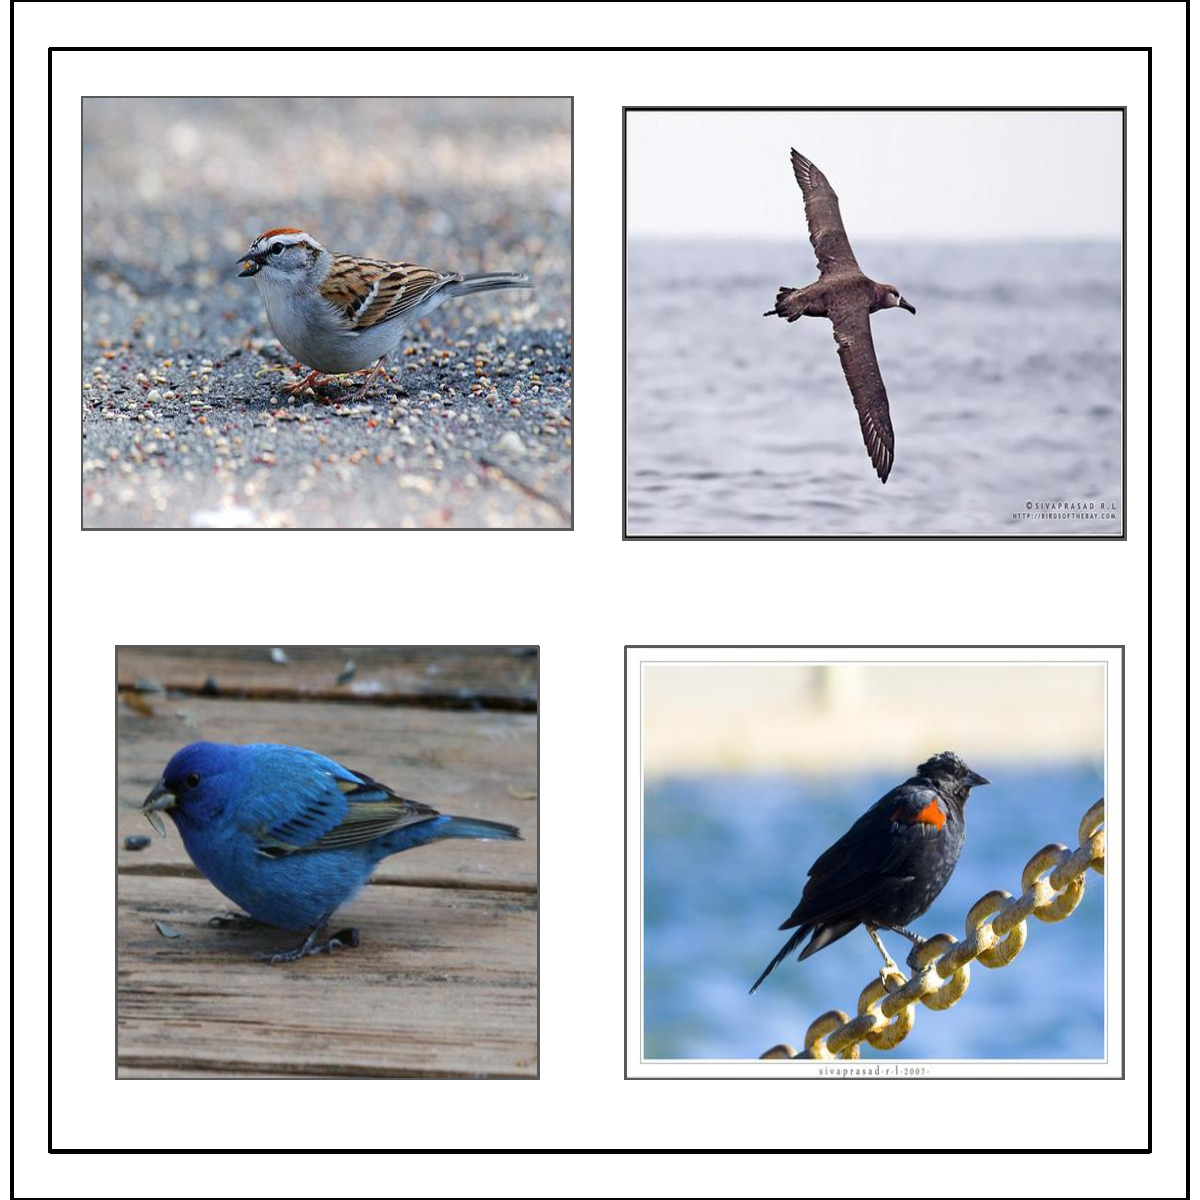
\includegraphics[width=\textwidth]{figures/Figure_3A.pdf}
  \subcaption{CUB dataset.}
\end{subfigure}
\hspace{0.04\textwidth}
% <— this is important. There should be no empty line here. 
\begin{subfigure}{0.25\textwidth}
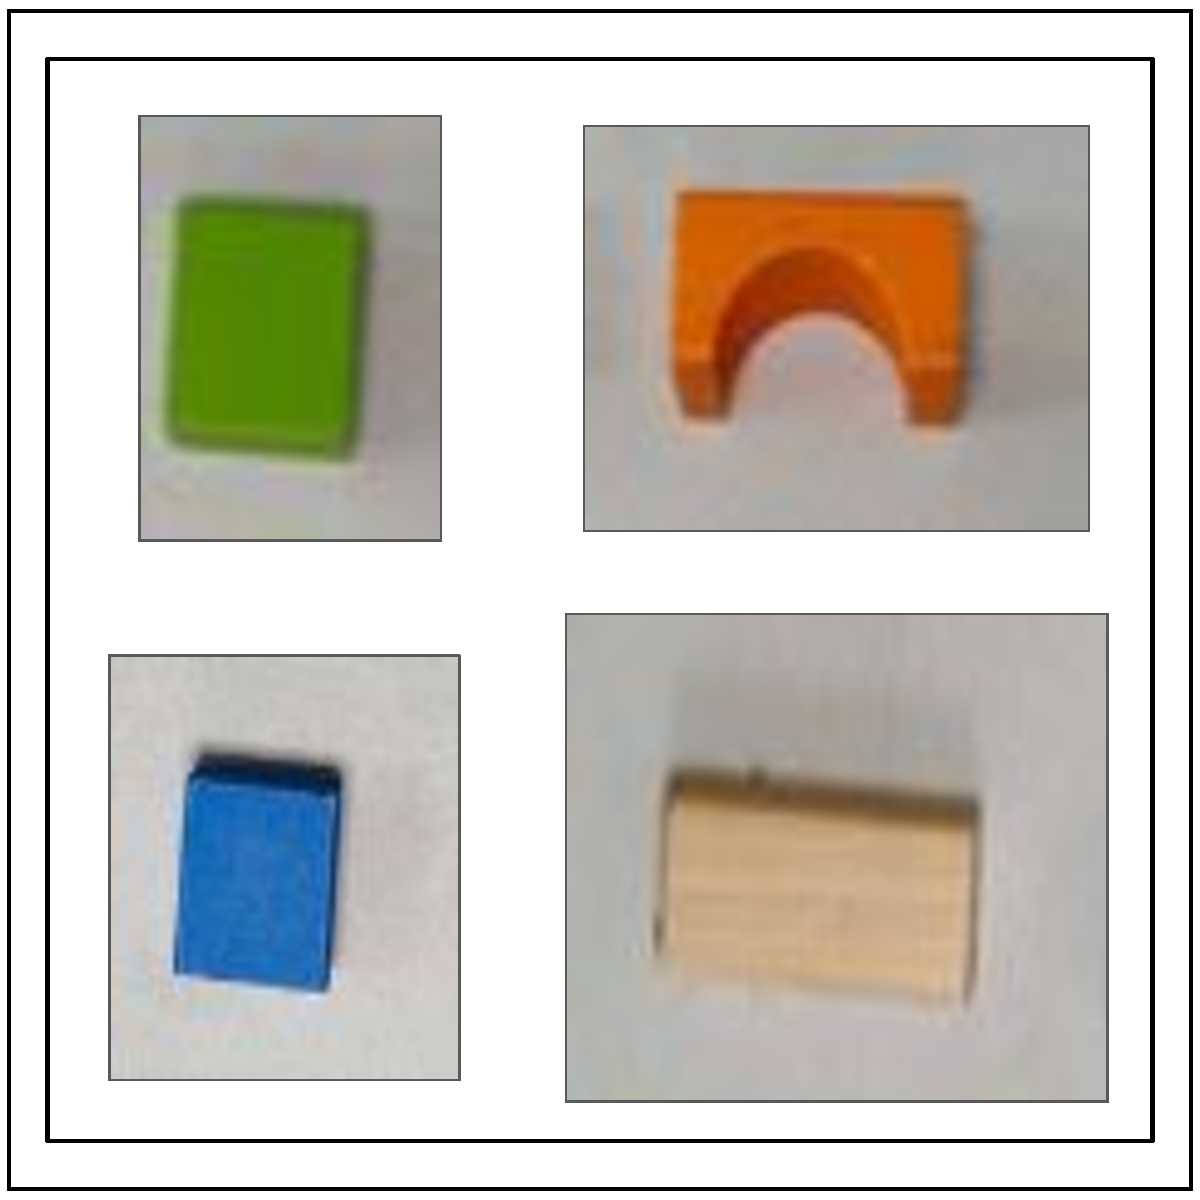
\includegraphics[width=\textwidth]{figures/Figure_3B.pdf}
  \subcaption{House construction domain}
\end{subfigure}
\hspace{0.04\textwidth}
%
\begin{subfigure}{0.25\textwidth}
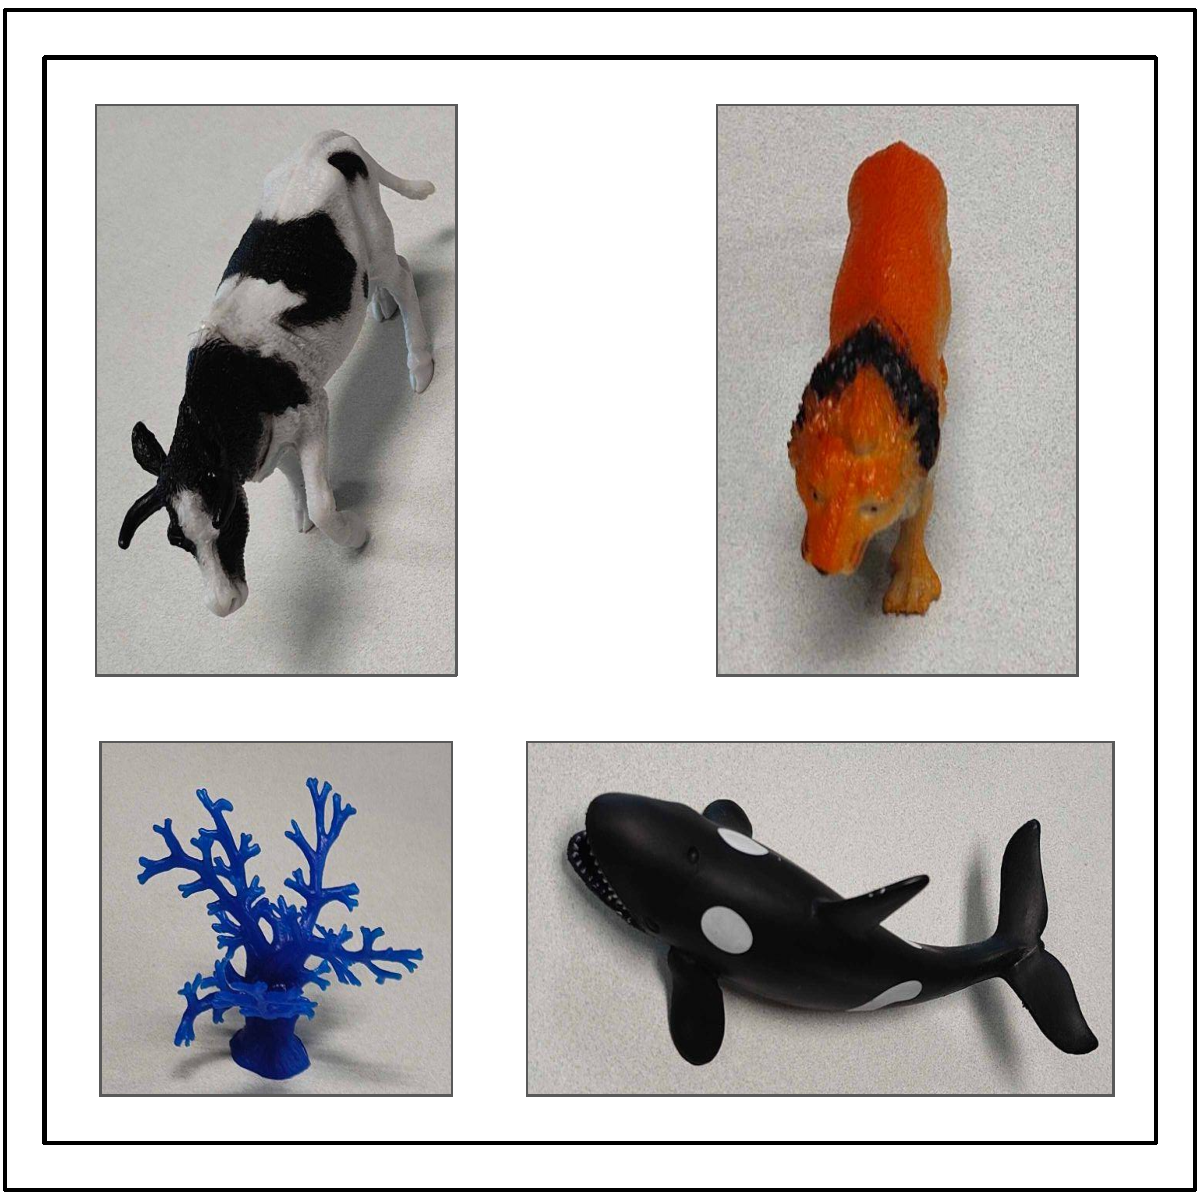
\includegraphics[width=\textwidth]{figures/Figure_3C.pdf}
  \subcaption{Zoo domain}
\end{subfigure}
\caption{Sample images from the three domains in this work.}
\label{fig:sampled_figures}
\end{figure*}


% \subsection{Node Classifier}
% Figure~\ref{fig:node_classifier} describes the process of how our pipeline choose an object to pick. 
% The inference is a two-step process, both using a BERT\textsubscript{base} model and a MLP layer, and taking the node context $t_i$ and he linguistic request $q$ as inputs.
% In the first step we use the BERT\textsubscript{base} model and a MLP layer to decide whether the node in the goal graph is different from the corresponding node in the demonstration. 
% Then we use another BERT\textsubscript{base} model and MLP layer to extract the object from $t_i$ and $q$ for this node location.

% In the example of Figure~\ref{fig:node_classifier}, we are trying to decide the object that should be placed in position $5$.
% Based on the node context $t_5$ and the request $q$, the node classifier decides that node $5$ in the goal graph should remain the same as the demonstration. 
% Then, we use the concept extractor to extract the object from $t_5$, and we found that the object that should be placed at node $5$ is ''blue rectangular tile''.

\subsection{Training Pipeline}
 We explain our training pipeline in this section. 
 The concepts from the dataset is divided into three groups: $C_{pretrain}, C_{train}$ and $C_{test}$, where the pre-train concepts $C_{pretrain}$ represent the pre-existing nodes in the knowledge graph. The training of the concept net model consists of three stages, the pre-training for the visual feature extractor, the pre-training for the embedding of pre-train concepts $C_{pretrain}$, and the training to update the knowledge graph with train concepts $C_{train}$. 
 \paragraph{Pre-training the Visual Feature Extractor.}
 In the first pre-training stage, we generate a VQA dataset on both the pre-train concepts $C_{pretrain}$ and the train concepts $C_{train}$. The purpose of this stage is to expose the visual feature extractor with a larger variation of visual features. 
 We jointly pre-train the visual feature extractor and the embedding for the pre-train concepts $C_{pretrain}$ and the train concepts $C_{train}$ with the visual question-answering task in this stage.
 After this pre-training stage, the embeddings of all pre-train concepts and train concepts will be discarded.
 \paragraph{Pre-training Pre-train Concepts.}
 The embedding of pre-train concepts $C_{pretrain}$ is obtained through gradient descent in this pre-train phase.
 For this phase, we generate a VQA dataset on the pre-train concepts $C_{pretrain}$ only.
 After we warmup the visual feature extractor in the first pre-training phase, we jointly train the visual feature extractor and the embedding for the pre-train concepts in this phase using the same VQA task.
 This pre-training step is skipped under the setting where the concept net has zero prior knowledge of the concepts, which is the setting of all of our experiments.
 \paragraph{Training.} 
 After we have pre-trained the visual feature extractor and the embedding for the pre-train concepts,  we train the concept learner module during the training stage.  We freeze the weights of the visual feature extractor at this stage because otherwise the embeddings for the pre-train concept will not be usable.  Because we hope to train ARGNN to update the embedding for known concepts with information from unseen instances, we have to reset the embedding for all the pre-train concepts and train concepts,$C_{pretrain}$ and $C_{train}$, after all the train concepts are inserted to the network.  After inserting all the concepts within the train set in the final round, we do not reset the embedding for the train concepts and insert the concepts in the test set $C_{test}$. 

\subsection{Training Configurations}
In this section we describe the training configuration of the experiments for all the three domains. 
During the training phase, the model completes one round of training if it finishes to insert all the concepts in the training set once. For simplicity, we unify the steps of training with rounds of insertion.
For all the experiment results we report in this work, we adopted the configuration where there is no pre-train concepts.
As a results, the second phase of pre-training is skipped for all the three datasets.
For all the three domains, we train our model for completing the concept graphs 100 rounds, and the number of concept insertions varies depending on the split of the concepts. We start the training with a learning rate of 0.001 and decrease the learning rate by a factor of 0.1 in every 25 rounds of completing the knowledge graph in the training stage.
For CUB-200-2011 dataset, we train our model for 50000 iterations with a batch size of 10. We use an Adam optimizer with learning rate of 0.0001 in the pre-training phase of the visual feature extractor.
For the house construction domain and the zoo domain, we train our model for 5000 iterations with a batch size of 10. We use an Adam optimizer with learning rate of 0.0001 in the pre-training stage of the visual feature extractor.

\subsection{Robot Setup}
We describe the details for camera calibration.
We need to calibrate cameras with respect to the FR3 base frame. 
We take multiple pictures in different configurations of the FR3 end-effector to which an acuro market is attached. This allows us to find a transformation matrix which converts the coordinates from the  camera frame to the robot base frame. The place scene camera is used to find the length of the object occupying the current node of the scene graph. 

We describe how we compute the placement location for each object in detailed.
SAM is used to segment the objects placed in the place scene and find the bounding boxes of each placed object which are also the nodes of our scene graph.
This allows us to calculate the position of the next object by finding the relative position of the next node with respect to the current object being placed.
, referencing the position of the node of the scene, and calculating the length of the bounding box of the referenced node. 
we use a formula of shift = 1/2*max(bounding box of the referenced node length)+50 pixel space \textbf{Next node position}= Relation to the reference node(Reference node position,shift). The function relation to the reference node adds a shift to the reference node position based on its relation to the next node. For example, it adds the shift only to the x coordinate if there is "to the top of" relation, or in the case of "to the right of" relation, it adds only the y coordinate of the current position. In our scene graph, we are able to identify "to the top of ", "to the bottom of"," to the right of"," to the left of", "to the top right of"," to the top left of"," to the bottom right of", and "to the bottom left of" relations.\\
The Segment Anything Model is capable of separating the foreground from the background. This allows us to find the table mask and the segment of each object placed in the camera frame on the table. \\
The flow of our pipeline requires us to first demonstrate the visual scene with all the objects placed in the Task scene to make a structure with linguistic inputs. 
We have to make sure that the objects are placed at a distance that allows SAM to create separate segment boxes for the objects. Then we pass each segmented object to either FALCON or Hi-Viscont classifiers to classify conditioned on the given language query. The robot then picks the object with simple visuo-motor servoing. 
by the node information of the scene graph. 
Once we find the object to be picked we then calculate the center of the bounding box of that object and convert it to the Robot frame with the help of the transformation matrix. 
If in the process there is an incomplete or erroneous grasp, we reattempt the whole classification again autonomously. Once the object is grasped we then place the object into the Task scene, with the position calculated relatively 
with respect to the previously placed object nodes or the ground. This process is iteratively done until we have completed the whole scene graph.
%\asnote{nodes in place of node or the ground} or \ngnote{the ground object}. 



\section{Dataset Statistics}\label{app:dataset_stats}
% \begin{table}[t]
% \resizebox{\columnwidth}{!}{%
% \begin{tabular}{c|ccc}
% \toprule
%     & Train & Test & Total\\
% \midrule
% CUB-200-2011 & $8232$ & $3556$ & $11788$  \\
% \midrule
% House& $217$ & $93$ & $310$\\
% \midrule
% Zoo& $196$ & $84$ & $280$\\
% \bottomrule
% \end{tabular}%
% }
% \caption{The number of images in the train and test split of each domain.}
% \label{tab:img_stats}
% \end{table}

% \begin{table}[t]
% \resizebox{\columnwidth}{!}{%
% \begin{tabular}{c|ccc}
% \toprule
%     & Train & Test & Total\\
% \midrule
% CUB & $307.8$ & $57.2$ & $365$  \\
% \midrule
% House& $34$ & $6$ & $40$\\
% \midrule
% Zoo& $28$ & $6$ & $34$\\
% \bottomrule
% \end{tabular}%
% }
% \caption{The number of concepts in the train and test split of each domain. The number of the CUB dataset comes from the average of five different splittings.}
% \label{tab:concept_stats}
% \end{table}

\begin{figure*}[h]
  \centering
\begin{subfigure}{0.28\textwidth}
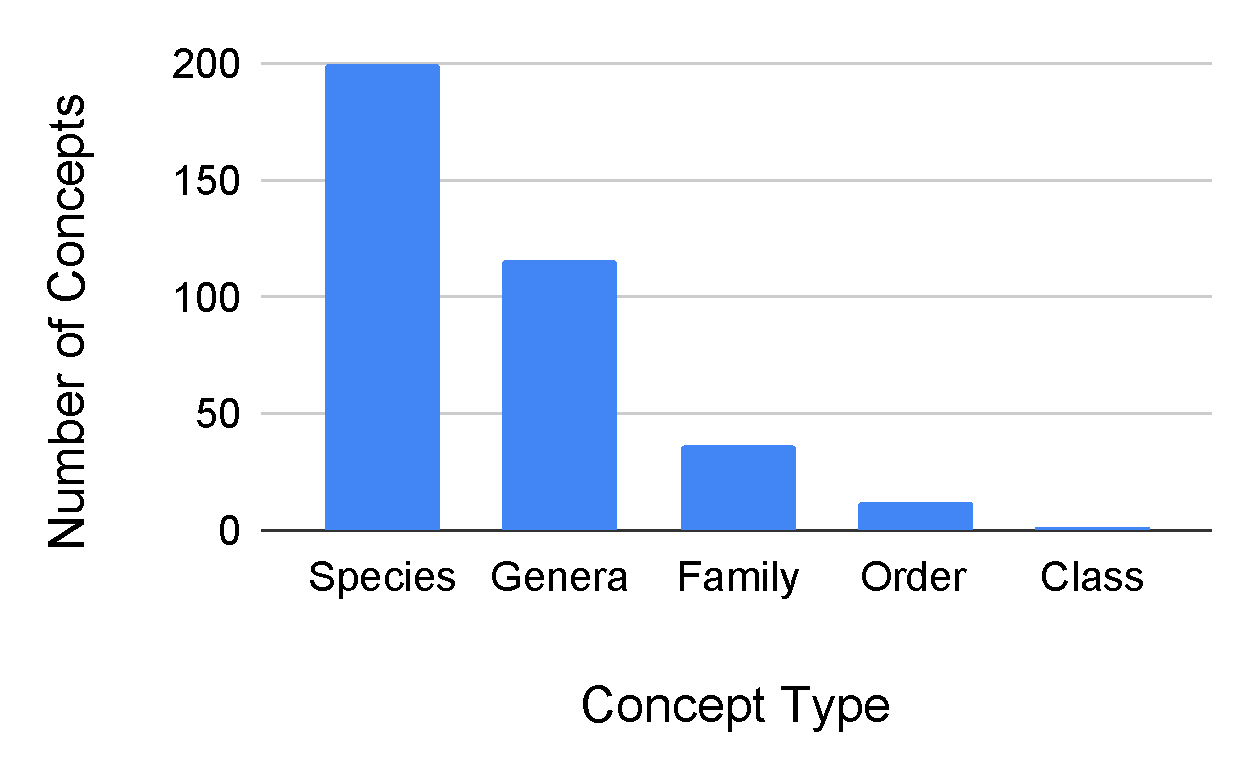
\includegraphics[width=\textwidth]{figures/chart_CUB.pdf}
  \subcaption{CUB-200-2011}
\end{subfigure}
\hspace{0.01\textwidth}
% <— this is important. There should be no empty line here. 
\begin{subfigure}{0.28\textwidth}
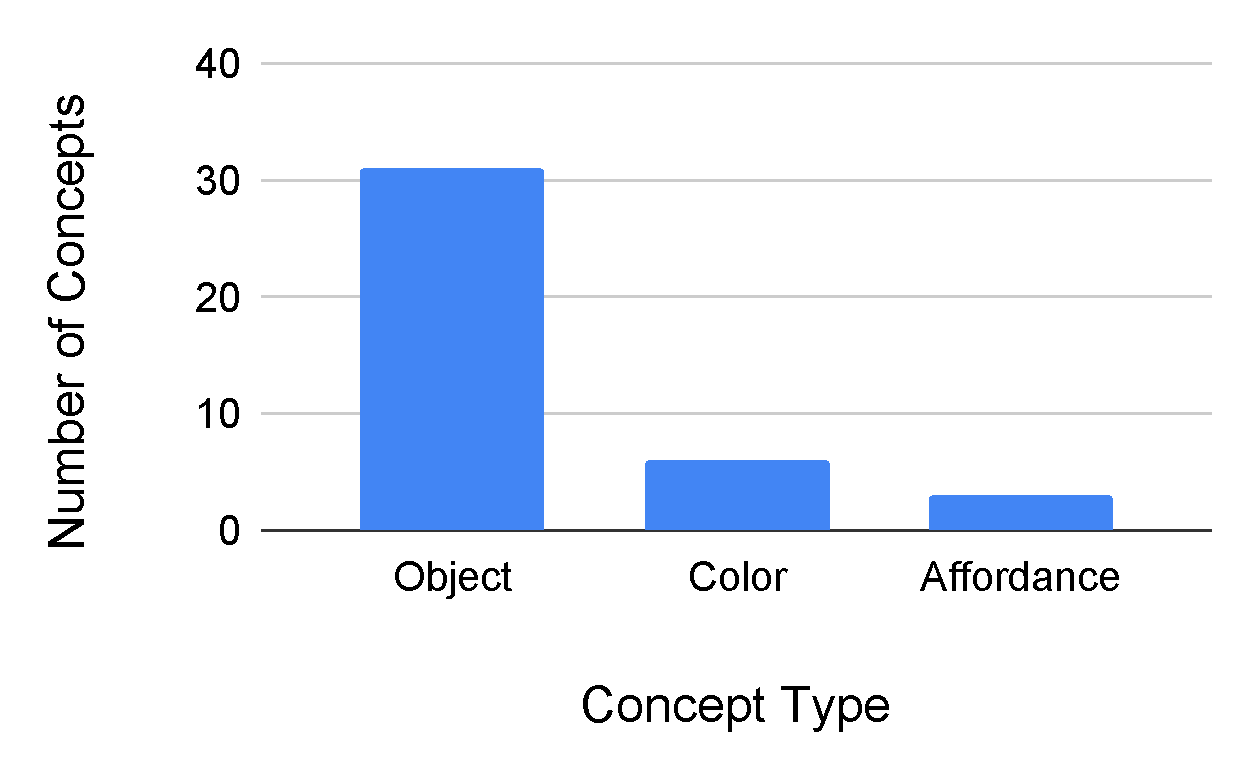
\includegraphics[width=\textwidth]{figures/chart_House.pdf}
  \subcaption{House Construction Domain}
\end{subfigure}
\hspace{0.01\textwidth}
%
\begin{subfigure}{0.28\textwidth}
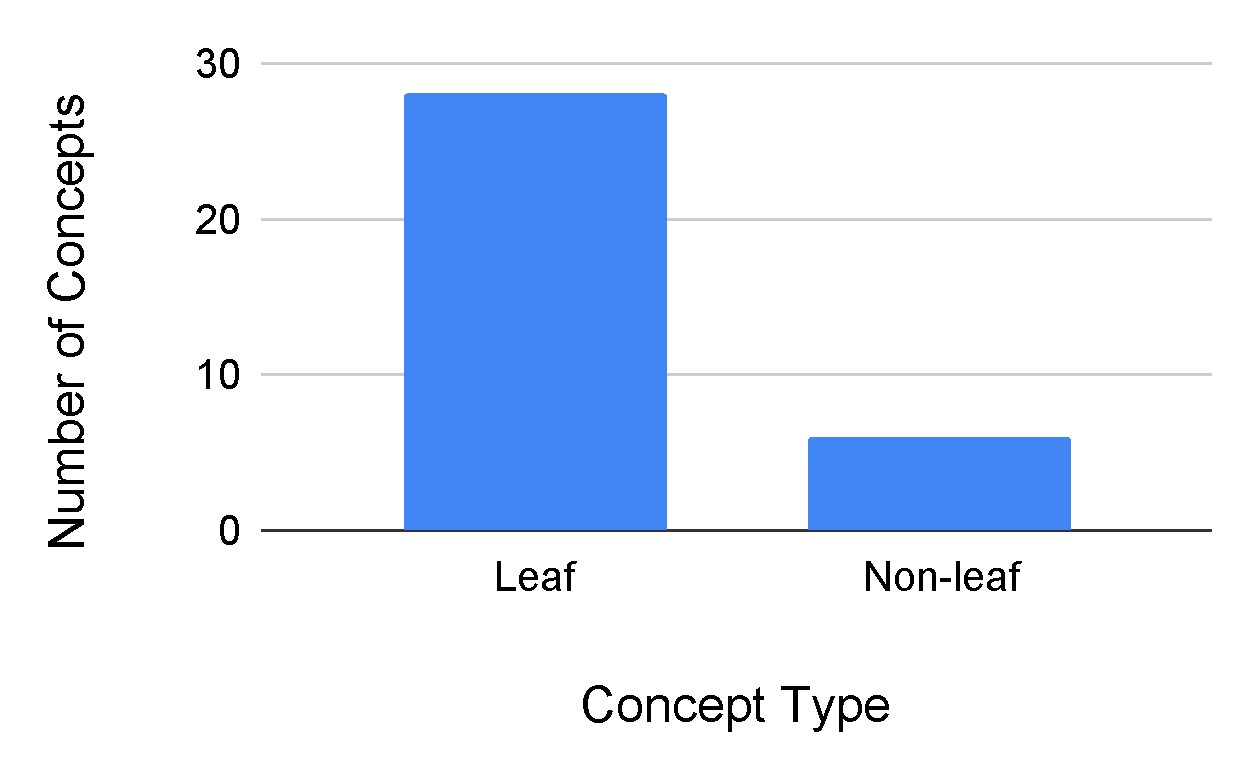
\includegraphics[width=\textwidth]{figures/chart_Zoo.pdf}
  \subcaption{Zoo Domain}
\end{subfigure}


\caption{The number of concepts of each type for all the three domains.}
\label{fig:concept_type}
\end{figure*}

\begin{table*}[t]
\resizebox{\textwidth}{!}{%
\begin{tabular}{c|ccc|ccc}
\toprule
    & Train Image & Test Image & Total Image& Train Concept & Test Concept & Total Concept\\
\midrule
CUB-200-2011 & $8232$ & $3556$ & $11788$ & $307.8$ & $58.2$ & $365$  \\
%\midrule
House& $217$ & $93$ & $310$& $34$ & $6$ & $40$\\
%\midrule
Zoo& $196$ & $84$ & $280$& $28$ & $6$ & $34$\\
\bottomrule
\end{tabular}%
}
\caption{Statistics for the three domains. The number of train and test concepts of the CUB-200-2011 dataset comes from the average of five different splits, resulted in decimal numbers.}
\label{tab:all_stats}
\end{table*}

We split our dataset at two different levels:- the level of concepts and the level of images. The images are divided into $70\%$ for training and $30\%$ for testing, and the testing images are used to evaluate for both seen and unseen concepts. At the concept level, we use five-fold validation. We train the model with $80\%$ of concepts and test on $20\%$ while covering all folds. Because the split of the non-leaf concepts need to guarantee that leaf concepts are unseen as well, our pick of the folds depends on the structure of the concept graph and is not as random as the regular five-fold validation.
The detailed descriptions of each domain are as follows:

\noindent\textbf{CUB-200-2011 dataset}\cite{WahCUB_200_2011} is a standard dataset to demonstrate visual concept learning.
It contains $11,788$ images for $200$ bird classes. Using the following  bird taxonomy\cite{Sullivan2009eBirdAC}, we added the hypernyms of the bird classes and used the bird taxonomy as the hierarchy of concepts.
Following the design of the dense graph propagation~\cite{kampffmeyer2019rethinking}, the relation of each concept includes all of its ancestors.
%Details of the concept relations will be provided in the supplementary materials.

\noindent\textbf{The house construction domain} includes $31$ types of building block objects.
Each object has $10$ different images. 
To introduce relations between concepts, we additionally add $6$ different concepts and $3$ different affordances of objects.
The dataset on the house construction domain includes $310$ images and $40$ concepts in total.
This domain is also used to train the models for the human subject study.
% fillout x from the dataset concepts


\noindent\textbf{The zoo domain} includes $28$ different types of objects. 
Similar to the house domain, we add $6$ general concepts to introduce a hierarchy for the concepts.
The dataset on the zoo domain includes $280$ images and $34$ concepts in total.

Additionally, the detailed statistics of image and concept of each split of each domain are presented in Table~\ref{tab:all_stats}, and the statistics of concept type are presented in Fig.~\ref{fig:concept_type}. Fig.~\ref{fig:sampled_figures} exhibits some sample images from the three domains.


\section{Detailed Results}\label{app:detailed_results}
\begin{table*}[t]
\resizebox{\textwidth}{!}{%
\begin{tabular}{c|cc|cc|cc}
\toprule
    & CUB-P & CUB-R & House-P& House-R & Zoo-P & Zoo-R \\
\midrule
Hi-Viscont & $91.03 \pm 3.00$ & $63.35\pm 9.69$ & $87.39\pm 1.71$  & $85.89\pm 9.95$ & $85.24\pm 5.41$ & $83.37\pm 15.67$\\
%\midrule
FALCON & $90.60\pm 4.18$  & $62.15\pm 8.38$  & $87.62\pm 1.71$ & $87.04\pm 8.29$ & $84.10\pm 5.86$& $87.41\pm 12.98$\\
\bottomrule
\end{tabular}%
}
\caption{The mean and standard deviation of precision and recall of Hi-Viscont and FALCON on the test concepts across all the three domains.}
\label{tab:detailed_test}
\end{table*}

\begin{table*}[t]
\resizebox{\textwidth}{!}{%
\begin{tabular}{c|cc|cc|cc|cc|cc}
\toprule
    &  Species-P& Species-R & Genera-P & Genera-R & Family-P & Family-R & Order-P & Order-R & Class-P & Class-R\\
\midrule
Hi-Viscont & $98.32\pm 0.63$  & $78.20\pm 3.56$ & $97.06\pm 0.44$ & $84.61\pm 0.90$ & $93.51\pm 2.33$& $88.12\pm 2.08$& $94.68\pm 1.58$& $89.40\pm 1.68$& $1\pm 0.00$ & $93.04\pm 13.71$\\
%\midrule
FALCON & $98.28\pm 0.59$ & $77.35\pm 2.59$& $96.66\pm 0.86$& $81.17\pm 1.24$ & $87.55\pm 3.13$& $81.43\pm 2.40$& $85.70\pm 3.70$& $83.10\pm 5.28$& $1\pm 0.00$ & $98.63\pm 1.85$ \\
\bottomrule
\end{tabular}%
}
\caption{The mean and standard deviation of precision and recall of the two models on CUB-200-2011 dataset by depth of concepts.}
\label{tab:detailed_CUB}
\end{table*}

\begin{table*}[t]
\resizebox{\textwidth}{!}{%
\begin{tabular}{c|cc|cc|cc}
\toprule
    & Object-P & Object-R & Color-P& Color-R & Affordance-P & Affordance-R \\
\midrule
Hi-Viscont & $86.19\pm 1.81$& $90.91\pm 3.08$& $99.94\pm 0.09$& $98.56\pm 1.41$& $95.51\pm 1.34$& $85.89\pm 14.86$\\
%\midrule
FALCON &$87.16\pm 1.43$& $91.57\pm 2.66$& $91.71\pm 2.28$& $83.80\pm 10.07$& $91.37\pm 1.71$& $42.25\pm 9.32$\\
\bottomrule
\end{tabular}%
}
\caption{The mean and standard deviation of precision and recall of the two models on the house domain by type of concepts.}
\label{tab:detailed_house}
\end{table*}

\begin{table*}[t]
\resizebox{\textwidth}{!}{%
\begin{tabular}{c|cc|cc}
\toprule
    & Leaf-P & Leaf-R & Non-leaf-P& Non-Leaf-R\\
\midrule
Hi-Viscont &$82.97\pm 5.32$& $93.89\pm 5.25$&$77.30\pm 7.77$& $96.93 \pm 5.97$\\
%\midrule
FALCON & $84.01\pm 5.29$& $94.90\pm 5.03$& $76.80\pm 4.08$& $58.38\pm 7.09$\\
\bottomrule
\end{tabular}%
}
\caption{The mean and standard deviation of precision and recall for the two models on the zoo domain by type of concepts.}
\label{tab:detailed_zoo}
\end{table*}

\subsection{Detailed Results on VQA}
We present the detailed results and analysis on VQA for each domain. Table~\ref{tab:detailed_test} presents the mean and standard deviation of the precision and recall of Hi-Viscont and FALCON on test concepts across all the three domains. The performance of both model is comparable on the test concepts on both precision and recall because majority of the test concepts are leaf concepts. Table~\ref{tab:detailed_CUB}, Table~\ref{tab:detailed_house}, and Table~\ref{tab:detailed_zoo} present the mean and standard deviation of the precision and recall for the CUB-200-2011 dataset, the house domain, and the zoo domain by the type of concept repectively. For all the three domains, Hi-Viscont consistently outperform FALCON on the recall metric for non-leaf concepts with a large margin because of the active updates from the ARGNN. Such results further demonstrate the importance of the information propagation from children to ancestor nodes in a continual learning setting.

\subsection{Statistic Tests on VQA}
In this section, we presents the statistic tests between Hi-Viscont and FALCON for all the three domains. 
\paragraph{CUB-200-2011.} Results of paired t-test suggest that Hi-Viscont achieves higher F1 scores with significance for concepts in Genera($p<0.001$), Family($p<0.001$), and Order($p=0.005$).
\paragraph{House Construction Domain.} Results of paired t-test suggests that Hi-Viscont achieves higher F1 scores with significance for color concepts($p=0.005$) and affordance concepts($p=0.002$).
\paragraph{Zoo Domain.} Results of paired t-test suggests that Hi-Viscont achieves higher F1 scores with significance for non-leaf concepts($p=0.001$).

%\ngnote{Conditions for normality were not met for the data points to run a t-test. Hence we conducted a Wilcoxon Signed-Rank test to compare .......}



\subsection{Detailed Results on Human Subject Experiments}
We present the results of statistical tests for each scale we measure for the human subject study in detailed in this subsection. 
For each metric, we report the results of a Shapiro-Wilk Normality test. If the data from such metric passes the normality test($p>0.05$), we report the results of a paired t-test.
Otherwise, we report the results of Wilcoxon signed rank test for that metric. 
\paragraph{Trust.} Results from Shapiro Wilk test suggest that our data in the Trust metric satisfies the condition for a parametric test($W=0.960, p=0.599$). Results from paired t-test suggest that Hi-Viscont is considered better than FALCON by users in the Trust metric with significance($t=2.325, p=0.016, df=17$).
\paragraph{SUS.} Results from Shapiro Wilk test suggest that our data in the SUS metric satisfies the condition for a parametric test($W=0.978, p=0.925$). Results from paired t-test suggest that Hi-Viscont is considered better than FALCON by users in the SUS metric with significance($t=2.428, p=0.013, df=17$).
\paragraph{Intelligence.}Results from Shapiro Wilk test suggest that our data in the Intelligence metric satisfies the condition for a parametric test($W=0.956, p=0.520$). Results from paired t-test suggest that Hi-Viscont is considered better than FALCON by users in the Intelligence metric with significance($t=2.591, p=0.010, df=17$).
\paragraph{Natural.}Results from Shapiro Wilk test suggest that our data in the Anthropomorphism metric satisfies the condition for a parametric test($W=0.937, p=0.255$). Results from paired t-test suggest that Hi-Viscont is considered better than FALCON by users in the Anthropomorphism metric with significance($t=2.924, p=0.005, df=17$).
\paragraph{Comparative.}Conditions for normality were not met for the data points to run a t-test. Hence we conducted a Wilcoxon Signed-Rank test to compare Hi-Viscont and FALCON in the comparative metric. Results from Wilcoxon signed-rank test suggest that Hi-Viscont is preferred by user in the direct comparison with FALCON with significance($Z=2.0, p<0.001$).
\paragraph{Success Rate.}Conditions for normality were not met for the data points to run a t-test. Hence we conducted a Wilcoxon Signed-Rank test to compare Hi-Viscont and FALCON in success rate. Results from Wilcoxon signed-rank test suggest that Hi-Viscont is better than FALCON in success rate with significance($Z=0.0, p=0.014$).
\paragraph{Node-level Accuracy.}Conditions for normality were not met for the data points to run a t-test. Hence we conducted a Wilcoxon Signed-Rank test to compare Hi-Viscont and FALCON in node-level accuracy. Results from Wilcoxon signed-rank test suggest that Hi-Viscont is better than FALCON in node-level accuracy with significance($Z=1.5, p=0.005$).




\end{document}
